% Created by tikzDevice version 0.10.1 on 2016-08-15 14:39:37
% !TEX encoding = UTF-8 Unicode
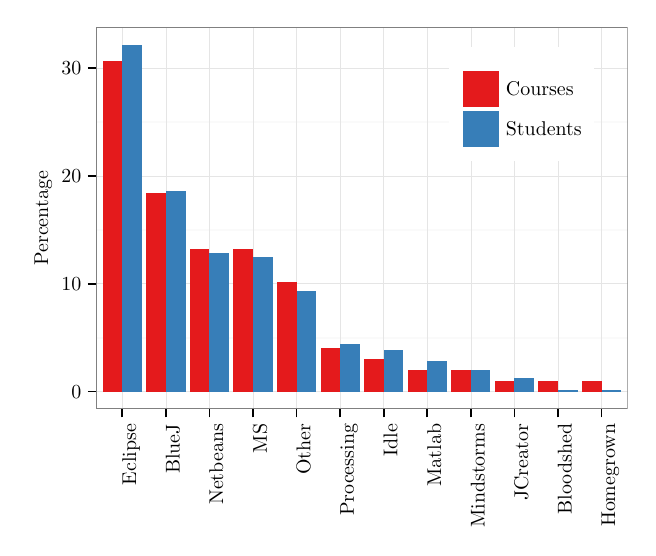
\begin{tikzpicture}[x=1pt,y=1pt]
\definecolor{fillColor}{RGB}{255,255,255}
\path[use as bounding box,fill=fillColor,fill opacity=0.00] (0,0) rectangle (216.81,180.67);
\begin{scope}
\path[clip] (  0.00,  0.00) rectangle (216.81,180.67);
\definecolor{drawColor}{RGB}{255,255,255}
\definecolor{fillColor}{RGB}{255,255,255}

\path[draw=drawColor,line width= 0.6pt,line join=round,line cap=round,fill=fillColor] (  0.00,  0.00) rectangle (216.81,180.68);
\end{scope}
\begin{scope}
\path[clip] ( 24.76, 42.89) rectangle (216.81,180.67);
\definecolor{fillColor}{RGB}{255,255,255}

\path[fill=fillColor] ( 24.76, 42.89) rectangle (216.81,180.67);
\definecolor{drawColor}{gray}{0.98}

\path[draw=drawColor,line width= 0.6pt,line join=round] ( 24.76, 68.65) --
	(216.81, 68.65);

\path[draw=drawColor,line width= 0.6pt,line join=round] ( 24.76,107.63) --
	(216.81,107.63);

\path[draw=drawColor,line width= 0.6pt,line join=round] ( 24.76,146.62) --
	(216.81,146.62);
\definecolor{drawColor}{gray}{0.90}

\path[draw=drawColor,line width= 0.2pt,line join=round] ( 24.76, 49.15) --
	(216.81, 49.15);

\path[draw=drawColor,line width= 0.2pt,line join=round] ( 24.76, 88.14) --
	(216.81, 88.14);

\path[draw=drawColor,line width= 0.2pt,line join=round] ( 24.76,127.13) --
	(216.81,127.13);

\path[draw=drawColor,line width= 0.2pt,line join=round] ( 24.76,166.11) --
	(216.81,166.11);

\path[draw=drawColor,line width= 0.2pt,line join=round] ( 34.20, 42.89) --
	( 34.20,180.67);

\path[draw=drawColor,line width= 0.2pt,line join=round] ( 49.94, 42.89) --
	( 49.94,180.67);

\path[draw=drawColor,line width= 0.2pt,line join=round] ( 65.69, 42.89) --
	( 65.69,180.67);

\path[draw=drawColor,line width= 0.2pt,line join=round] ( 81.43, 42.89) --
	( 81.43,180.67);

\path[draw=drawColor,line width= 0.2pt,line join=round] ( 97.17, 42.89) --
	( 97.17,180.67);

\path[draw=drawColor,line width= 0.2pt,line join=round] (112.91, 42.89) --
	(112.91,180.67);

\path[draw=drawColor,line width= 0.2pt,line join=round] (128.65, 42.89) --
	(128.65,180.67);

\path[draw=drawColor,line width= 0.2pt,line join=round] (144.40, 42.89) --
	(144.40,180.67);

\path[draw=drawColor,line width= 0.2pt,line join=round] (160.14, 42.89) --
	(160.14,180.67);

\path[draw=drawColor,line width= 0.2pt,line join=round] (175.88, 42.89) --
	(175.88,180.67);

\path[draw=drawColor,line width= 0.2pt,line join=round] (191.62, 42.89) --
	(191.62,180.67);

\path[draw=drawColor,line width= 0.2pt,line join=round] (207.36, 42.89) --
	(207.36,180.67);
\definecolor{fillColor}{RGB}{228,26,28}

\path[fill=fillColor] ( 27.12, 49.15) rectangle ( 34.20,168.50);
\definecolor{fillColor}{RGB}{55,126,184}

\path[fill=fillColor] ( 34.20, 49.15) rectangle ( 41.29,174.41);
\definecolor{fillColor}{RGB}{228,26,28}

\path[fill=fillColor] ( 42.86, 49.15) rectangle ( 49.94,120.76);
\definecolor{fillColor}{RGB}{55,126,184}

\path[fill=fillColor] ( 49.94, 49.15) rectangle ( 57.03,121.70);
\definecolor{fillColor}{RGB}{228,26,28}

\path[fill=fillColor] ( 58.60, 49.15) rectangle ( 65.69,100.87);
\definecolor{fillColor}{RGB}{55,126,184}

\path[fill=fillColor] ( 65.69, 49.15) rectangle ( 72.77, 99.10);
\definecolor{fillColor}{RGB}{228,26,28}

\path[fill=fillColor] ( 74.34, 49.15) rectangle ( 81.43,100.87);
\definecolor{fillColor}{RGB}{55,126,184}

\path[fill=fillColor] ( 81.43, 49.15) rectangle ( 88.51, 97.64);
\definecolor{fillColor}{RGB}{228,26,28}

\path[fill=fillColor] ( 90.09, 49.15) rectangle ( 97.17, 88.94);
\definecolor{fillColor}{RGB}{55,126,184}

\path[fill=fillColor] ( 97.17, 49.15) rectangle (104.25, 85.66);
\definecolor{fillColor}{RGB}{228,26,28}

\path[fill=fillColor] (105.83, 49.15) rectangle (112.91, 65.07);
\definecolor{fillColor}{RGB}{55,126,184}

\path[fill=fillColor] (112.91, 49.15) rectangle (120.00, 66.50);
\definecolor{fillColor}{RGB}{228,26,28}

\path[fill=fillColor] (121.57, 49.15) rectangle (128.65, 61.09);
\definecolor{fillColor}{RGB}{55,126,184}

\path[fill=fillColor] (128.65, 49.15) rectangle (135.74, 64.19);
\definecolor{fillColor}{RGB}{228,26,28}

\path[fill=fillColor] (137.31, 49.15) rectangle (144.40, 57.11);
\definecolor{fillColor}{RGB}{55,126,184}

\path[fill=fillColor] (144.40, 49.15) rectangle (151.48, 60.07);
\definecolor{fillColor}{RGB}{228,26,28}

\path[fill=fillColor] (153.05, 49.15) rectangle (160.14, 57.11);
\definecolor{fillColor}{RGB}{55,126,184}

\path[fill=fillColor] (160.14, 49.15) rectangle (167.22, 56.92);
\definecolor{fillColor}{RGB}{228,26,28}

\path[fill=fillColor] (168.80, 49.15) rectangle (175.88, 53.13);
\definecolor{fillColor}{RGB}{55,126,184}

\path[fill=fillColor] (175.88, 49.15) rectangle (182.96, 54.01);
\definecolor{fillColor}{RGB}{228,26,28}

\path[fill=fillColor] (184.54, 49.15) rectangle (191.62, 53.13);
\definecolor{fillColor}{RGB}{55,126,184}

\path[fill=fillColor] (191.62, 49.15) rectangle (198.71, 49.76);
\definecolor{fillColor}{RGB}{228,26,28}

\path[fill=fillColor] (200.28, 49.15) rectangle (207.36, 53.13);
\definecolor{fillColor}{RGB}{55,126,184}

\path[fill=fillColor] (207.36, 49.15) rectangle (214.45, 49.76);
\definecolor{drawColor}{gray}{0.50}

\path[draw=drawColor,line width= 0.6pt,line join=round,line cap=round] ( 24.76, 42.89) rectangle (216.81,180.67);
\end{scope}
\begin{scope}
\path[clip] (  0.00,  0.00) rectangle (216.81,180.67);
\definecolor{drawColor}{RGB}{0,0,0}

\node[text=drawColor,anchor=base east,inner sep=0pt, outer sep=0pt, scale=  0.72] at ( 19.36, 46.67) {0};

\node[text=drawColor,anchor=base east,inner sep=0pt, outer sep=0pt, scale=  0.72] at ( 19.36, 85.66) {10};

\node[text=drawColor,anchor=base east,inner sep=0pt, outer sep=0pt, scale=  0.72] at ( 19.36,124.65) {20};

\node[text=drawColor,anchor=base east,inner sep=0pt, outer sep=0pt, scale=  0.72] at ( 19.36,163.63) {30};
\end{scope}
\begin{scope}
\path[clip] (  0.00,  0.00) rectangle (216.81,180.67);
\definecolor{drawColor}{RGB}{0,0,0}

\path[draw=drawColor,line width= 0.6pt,line join=round] ( 21.76, 49.15) --
	( 24.76, 49.15);

\path[draw=drawColor,line width= 0.6pt,line join=round] ( 21.76, 88.14) --
	( 24.76, 88.14);

\path[draw=drawColor,line width= 0.6pt,line join=round] ( 21.76,127.13) --
	( 24.76,127.13);

\path[draw=drawColor,line width= 0.6pt,line join=round] ( 21.76,166.11) --
	( 24.76,166.11);
\end{scope}
\begin{scope}
\path[clip] (  0.00,  0.00) rectangle (216.81,180.67);
\definecolor{drawColor}{RGB}{0,0,0}

\path[draw=drawColor,line width= 0.6pt,line join=round] ( 34.20, 39.89) --
	( 34.20, 42.89);

\path[draw=drawColor,line width= 0.6pt,line join=round] ( 49.94, 39.89) --
	( 49.94, 42.89);

\path[draw=drawColor,line width= 0.6pt,line join=round] ( 65.69, 39.89) --
	( 65.69, 42.89);

\path[draw=drawColor,line width= 0.6pt,line join=round] ( 81.43, 39.89) --
	( 81.43, 42.89);

\path[draw=drawColor,line width= 0.6pt,line join=round] ( 97.17, 39.89) --
	( 97.17, 42.89);

\path[draw=drawColor,line width= 0.6pt,line join=round] (112.91, 39.89) --
	(112.91, 42.89);

\path[draw=drawColor,line width= 0.6pt,line join=round] (128.65, 39.89) --
	(128.65, 42.89);

\path[draw=drawColor,line width= 0.6pt,line join=round] (144.40, 39.89) --
	(144.40, 42.89);

\path[draw=drawColor,line width= 0.6pt,line join=round] (160.14, 39.89) --
	(160.14, 42.89);

\path[draw=drawColor,line width= 0.6pt,line join=round] (175.88, 39.89) --
	(175.88, 42.89);

\path[draw=drawColor,line width= 0.6pt,line join=round] (191.62, 39.89) --
	(191.62, 42.89);

\path[draw=drawColor,line width= 0.6pt,line join=round] (207.36, 39.89) --
	(207.36, 42.89);
\end{scope}
\begin{scope}
\path[clip] (  0.00,  0.00) rectangle (216.81,180.67);
\definecolor{drawColor}{RGB}{0,0,0}

\node[text=drawColor,rotate= 90.00,anchor=base east,inner sep=0pt, outer sep=0pt, scale=  0.72] at ( 39.16, 37.49) {Eclipse};

\node[text=drawColor,rotate= 90.00,anchor=base east,inner sep=0pt, outer sep=0pt, scale=  0.72] at ( 54.90, 37.49) {BlueJ};

\node[text=drawColor,rotate= 90.00,anchor=base east,inner sep=0pt, outer sep=0pt, scale=  0.72] at ( 70.65, 37.49) {Netbeans};

\node[text=drawColor,rotate= 90.00,anchor=base east,inner sep=0pt, outer sep=0pt, scale=  0.72] at ( 86.39, 37.49) {MS};

\node[text=drawColor,rotate= 90.00,anchor=base east,inner sep=0pt, outer sep=0pt, scale=  0.72] at (102.13, 37.49) {Other};

\node[text=drawColor,rotate= 90.00,anchor=base east,inner sep=0pt, outer sep=0pt, scale=  0.72] at (117.87, 37.49) {Processing};

\node[text=drawColor,rotate= 90.00,anchor=base east,inner sep=0pt, outer sep=0pt, scale=  0.72] at (133.61, 37.49) {Idle};

\node[text=drawColor,rotate= 90.00,anchor=base east,inner sep=0pt, outer sep=0pt, scale=  0.72] at (149.36, 37.49) {Matlab};

\node[text=drawColor,rotate= 90.00,anchor=base east,inner sep=0pt, outer sep=0pt, scale=  0.72] at (165.10, 37.49) {Mindstorms};

\node[text=drawColor,rotate= 90.00,anchor=base east,inner sep=0pt, outer sep=0pt, scale=  0.72] at (180.84, 37.49) {JCreator};

\node[text=drawColor,rotate= 90.00,anchor=base east,inner sep=0pt, outer sep=0pt, scale=  0.72] at (196.58, 37.49) {Bloodshed};

\node[text=drawColor,rotate= 90.00,anchor=base east,inner sep=0pt, outer sep=0pt, scale=  0.72] at (212.32, 37.49) {Homegrown};
\end{scope}
\begin{scope}
\path[clip] (  0.00,  0.00) rectangle (216.81,180.67);
\definecolor{drawColor}{RGB}{0,0,0}

\node[text=drawColor,rotate= 90.00,anchor=base,inner sep=0pt, outer sep=0pt, scale=  0.72] at (  7.36,111.78) {Percentage};
\end{scope}
\begin{scope}
\path[clip] (  0.00,  0.00) rectangle (216.81,180.67);
\definecolor{fillColor}{RGB}{255,255,255}

\path[fill=fillColor] (152.28,132.59) rectangle (204.51,173.65);
\end{scope}
\begin{scope}
\path[clip] (  0.00,  0.00) rectangle (216.81,180.67);
\definecolor{fillColor}{RGB}{228,26,28}

\path[fill=fillColor] (157.26,152.02) rectangle (170.30,165.05);
\end{scope}
\begin{scope}
\path[clip] (  0.00,  0.00) rectangle (216.81,180.67);
\definecolor{fillColor}{RGB}{55,126,184}

\path[fill=fillColor] (157.26,137.57) rectangle (170.30,150.60);
\end{scope}
\begin{scope}
\path[clip] (  0.00,  0.00) rectangle (216.81,180.67);
\definecolor{drawColor}{RGB}{0,0,0}

\node[text=drawColor,anchor=base west,inner sep=0pt, outer sep=0pt, scale=  0.72] at (172.81,156.06) {Courses};
\end{scope}
\begin{scope}
\path[clip] (  0.00,  0.00) rectangle (216.81,180.67);
\definecolor{drawColor}{RGB}{0,0,0}

\node[text=drawColor,anchor=base west,inner sep=0pt, outer sep=0pt, scale=  0.72] at (172.81,141.61) {Students};
\end{scope}
\end{tikzpicture}
